%!TEX root = exam.tex
\begin{center}
    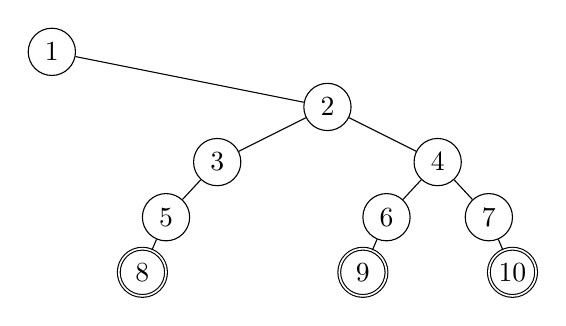
\begin{tikzpicture}[level distance=0.7cm,
        level 1/.style={sibling distance=7cm},
        level 2/.style={sibling distance=2.8cm},
        level 3/.style={sibling distance=1.3cm},
        level 4/.style={sibling distance=0.6cm},
        level 5/.style={sibling distance=0.2cm},
        every node/.style={draw,circle,inner sep=0pt,minimum size=6mm}]
        \node {1}
        child[missing]
        child {
            node {2}
            child {
                node {3}
                child {
                    node {5}
                    child {
                        node[double]{8}
                    }
                    child[missing]
                }
                child[missing]
            }
            child {
                node {4}
                child {
                    node {6}
                    child {
                        node[double]{9}
                    }
                    child[missing]
                }
                child {
                    node {7}
                    child[missing]
                    child {
                        node[double]{10}
                    }
                }
            }
        }
        ;
    \end{tikzpicture}
\end{center}